%It is recommended that you use pdflatex for compilation

\documentclass[10pt,letterpaper]{article}

\usepackage[pdftex]{graphicx}
%\usepackage{fullpage} % reduces margins if uncommented

\usepackage{hyperref}
\newcommand{\urlfootnote}[1]{\footnote{\url{#1}}}
\newcommand{\code}[1]{\par\texttt{#1}\par}

\title{CBCJVM --- Applications of the Java Virtual Machine with Robotics}
\author{Braden McDorman (braden@betabot.org)\\
Benjamin Woodruff (odetopi.e@gmail.com)\\
Akshay Joshi (me@akshayjoshi.com)\\
Jonathan Frias (freakinjonathan@gmail.com)}
%we should clean up the way the author list is formated

\begin{document}

\maketitle

\section{Concept and Background}

\subsection{Thesis}

The Botball tournament requires programmers to rapidly develop and prototype programs. However a disconnect is visible between the language and the tools provided and the goals of the game. Although very fast, C is generally considered to be a low-level language, making it what many of us believe to be the wrong tool for the job. The result is buggy programs, cluttered code, and a lack of flexibility in user libraries. The CBCJVM is the product of the realization that although slower, interpreted Object-Oriented programming languages are better for the type of prototyping used in the Botball competition. As Kipr has stated many times, it is highly unlikely that the CBC will ever be officially changed from C \urlfootnote{http://community.botball.org/forum/miscellaneous/suggestions-and-bugs/can-there-be-kiss-c-rather-kiss-c}. CBCJVM shares many of the same goals as Nease's CBCLua, but it is aimed at a wider audience, with monthly releases, detailed documentation, and support for more than just one language. CBCJVM is not just a port of JVM to the CBC, but it encompasses a group of libraries and tools to compete with (and often times surpass) those offered by KISS-C.



\subsection{License}

CBCJVM is licensed under the GPLv3\urlfootnote{http://gplv3.fsf.org/}. This license requires that you distribute the source code of any modifications of CBCJVM along with any binary version of it that you distribute. We, the authors of CBCJVM, believe this constitutes a fair and just agreement. You are also permitted to use CBCJVM under any future version of the GPL that you wish.



\subsection{Languages}

The CBCJVM originally went under the name ``CBCJava", but as the project grew, it was soon realized that using the JVM only for Java was a waste. The Java Virtual Machine has become a de facto standard of virtual machines, and almost every interpreted language imaginable has some port to the JVM, and these languages typically have support for interfacing with Java libraries. The JVM is fast, taking advantage of Just-In-Time compilation and various other optimizations, making it's performance somewhat comparable to C++ and C (but performance is still in no way better than a native language). CBCJVM has been used with JavaScript (via Mozilla Rhino) and Scala (which compiles directly to Java byte-code), but it can be used with many other languages such as Ruby, Python, Lua, and even LOLCODE. While it cannot match the performance of native interpreters for these languages, such as WebKit (JavaScript), CPython, or the standard Lua interpreter, it offers a fast way for these teams to get up and running with these high level languages. What's more, is that CBCJVM already includes a set of powerful libraries that can be used in conjunction with these languages to help teams that would otherwise be on their own with a language. (Not everyone can port and develop libraries in a language entirely by themselves and have it work well... *cough* Nease, CBCLua *cough*)



\subsection{Libraries}

Rather than being a straight port of the JVM to the CBC, CBCJVM includes libraries developed on top of the JVM. These libraries allow access to the KISS-C libraries via the Java Native Interface (JNI), allowing you to control motors, read sensors, and so on. Although bugs occasionally show up in this low-level communication layer, we believe that our implementation is complete and stable enough to be used on a day-to-day basis. These low level functions are available in the \texttt{cbccore.low} package.

On top of this, we have classes that make the low level functions more object-oriented, and use camelCase for function names, rather than KISS-C's underscore{\_}naming{\_}system. The majority of CBCJVM's classes use these camelCased classes, and so should you. That said, All simulation happens in this \texttt{cbccore.low} package, and thus there is not loss in functionality by using the \texttt{cbccore.low} package. There exist two obvious reasons for the use of the \texttt{cbccore.low} package in your own code:
\begin{itemize}
\item Ease of porting from KISS-C code.

\textit{Although the best option would be to port your code to CBCJVM utilizing the new APIs, in an object-oriented fashion, the \textit{cbccore.low} package can be used to do a quick ad-hoc port of code, due to it's similarities to the KISS-C's API.}

\item The use of some feature where no high-level, camelCased class exists to handle it yet.

\textit{We try our best, but as a (currently) small development team, there is the possibility that we have overlooked some functions in our porting efforts. However, the best option would be to fork\urlfootnote{http://help.github.com/forking} our github repository\urlfootnote{http://github.com/catron/CBCJVM}, add that functionality yourself, and submit a pull request\urlfootnote{http://github.com/guides/pull-requests}, or report it in our github issue tracker \urlfootnote{http://github.com/catron/CBCJVM/issues} and wait for a fix.}
\end{itemize}

\pagebreak

\section{Features and Internals}

\subsection{Running the JVM}
CBCJVM uses a lightweight JVM called JamVM\urlfootnote{http://jamvm.sourceforge.net/}. JamVM is designed for embedded platforms, such as the Linux running Chumby used in the CBC. JamVM gives us excellent compatibility with Sun's Java standard library because it uses GNU Classpath\urlfootnote{http://www.gnu.org/software/classpath/} for it's standard library. This allows us to run generated byte code on the computer and CBC with no modification. Our simulator exploits this cross compatibility by replacing the \texttt{cbccore.low.*} libraries at runtime.

\subsection{Simulator}
As mentioned, our simulator replaces classes loaded by \texttt{cbccore.Device} at runtime if it detects it is running on a computer. These simulated Device classes then update a Simulator GUI singleton.

\subsection{Frame Buffer Access}
One of the more unique features of CBCJVM is the ability to draw to the CBC's 320x240 screen. This is accomplished by writing RGB16 data to the \textsl{/dev/fb0} pipe provided by Linux. A custom-made library built specifically for CBCJVM gives you helper classes such as pixmaps (Pixel Buffers) with drawing functions and Image data types. The frame buffer is also simulated on the computer, allowing you to test your drawing code directly in the simulator. You can find more details about CBCJVM's frame buffer library in \texttt{cbccore.display} package.

\subsection{Configuration System}
``Configurators" can get input from a user for several options using buttons, touch sensors, or even analog sensors using an \texttt{cbcccore.sensors.analog.AnalogBooleanAdapter}. This is accomplished by passing an array of options along with an array of acceptable \texttt{IBooleanSensor}s to use, then mapping each option to a unique sensor. Using Configurators allows a programmer to quickly build menu systems based off of the inputs their robot can handle.

\subsection{Eclipse Integration}
Ease of use being of the utmost importance to our team, CBCJVM’s Eclipse\urlfootnote{http://www.eclipse.org/} Plugin allows you to download to your CBC via a network or via a flash drive. Eclipse's built in documentation, code completion, and automatic build system allow for you to develop code even faster. Eclipse also provides thousands of plugins for things such as version control with git and svn. When downloading over the network there is no need to recompile your program, just simply press run again.

\pagebreak
\section{Usage}

\subsection{Setup}

\subsubsection{Background Information}

Currently, the only supported platform is Ubuntu Linux. The instructions are untested with other distros, but they should work with slight modifications (eg.\ \texttt{yum} on RedHat/CentOS/Fedora instead of \texttt{apt-get}, and equivalent package names). On MacOS X Java 6 is poorly supported, and may or may not run on your machine\urlfootnote{http://java.dzone.com/news/java-6-mac-worsest-release-eve}. You might be better off trying to modify CBCJVM to work under Java 5 or using a virtual machine to run Ubuntu on top of your machine for builds (we recommend the free VirtualBox\urlfootnote{http://www.virtualbox.org/}). On Windows, everything should work, except for the few bash-based build scripts (the build process is mainly Ant and Maven based). Windows support is a priority, and should be an easy project for anyone who wishes to take on the task.

\textbf{Warning: } Build instructions may change over time. Therefore, it is always a good idea to consult the CBCJVM wiki\urlfootnote{http://wiki.github.com/catron/CBCJVM/installsetup} for the latest information.

\subsubsection{Ubuntu Setup}

All of these commands, unless otherwise specified, are to be executed in a bash (terminal) environment. On a fresh Ubuntu install, that would be found under the top left ``Applications" menu, ``Accessories", ``Terminal". If a command asks for your password, it is referring to your root (administrative) password. If you have no idea what this means, please contact your system administrator.
\begin{enumerate}
\item Open the ``Software Sources" application by going to the ``System" menu at the top left of your screen, ``Administration", ``Software Sources"
\item Ensure the box ``Community-maintained Open Source software (universe)" is checked, if not, check it.
\item Close the window. If you are prompted to update your package list, click the ``Reload" button.
\item Check and see if you have a copy of JDK 6 by running:
      \code{\$ javac -version}
      You should see something like:
      \code{\$ javac 1.6.0{\_}18}
      If it gives a version prior to 1.6.x{\_}x, update your system. If it complain that javac is not found, run
      \code{\$ sudo apt-get install default-jdk}
\item Now, install the additional dependencies:
      \code{\$ sudo apt-get install ant git-core maven2}
      If you already have one of those pieces of software, you can still run the command without fear. Aptitude won't attempt to reinstall the software.
\item Navigate into the directory you want the repository folder to be downloaded to:
      \code{\$ cd "/directory/on/drive"}
      Pull (download) a copy of CBCJVM:\par
      \begin{itemize}
          \item Download the latest version (possibly unstable):
                \code{\$ git clone git://github.com/catron/CBCJVM.git \\
                      \$ cd CBCJVM}
          \item Download a specific (``stable") version:
                \code{\$ git clone git://github.com/catron/CBCJVM.git \\
                      \$ cd CBCJVM \\
                      \$ git tag -l \\
                      \$ git checkout 10.6}
                (\texttt{git tag -l} is optional, it will list all available versions. Replace `10.6' with whatever version number you desire.)
      \end{itemize}
      If you are unsure as to what version you should download, it is recommended that you consult someone on the Botball community chat\urlfootnote{http://community.botball.org/irc}.
\item Compile CBCJVM:
      \code{\$ sh BuildEverything.sh}
\item The CBC installer and corresponding README file can now be found in \texttt{CBCJVM/installer/install}.
\end{enumerate}



\subsection{Finding Documentation with JavaDoc}

After running the build script, a series of HTML pages will be generated in \texttt{CBCJVM/cbc/CBCJVM/doc}. You can open the file \texttt{index.html} from that directory with your favorite web-browser. This documentation is automatically generated from the CBCJVM source code, and is rebuilt with each execution of the build script.

\begin{figure}[h]
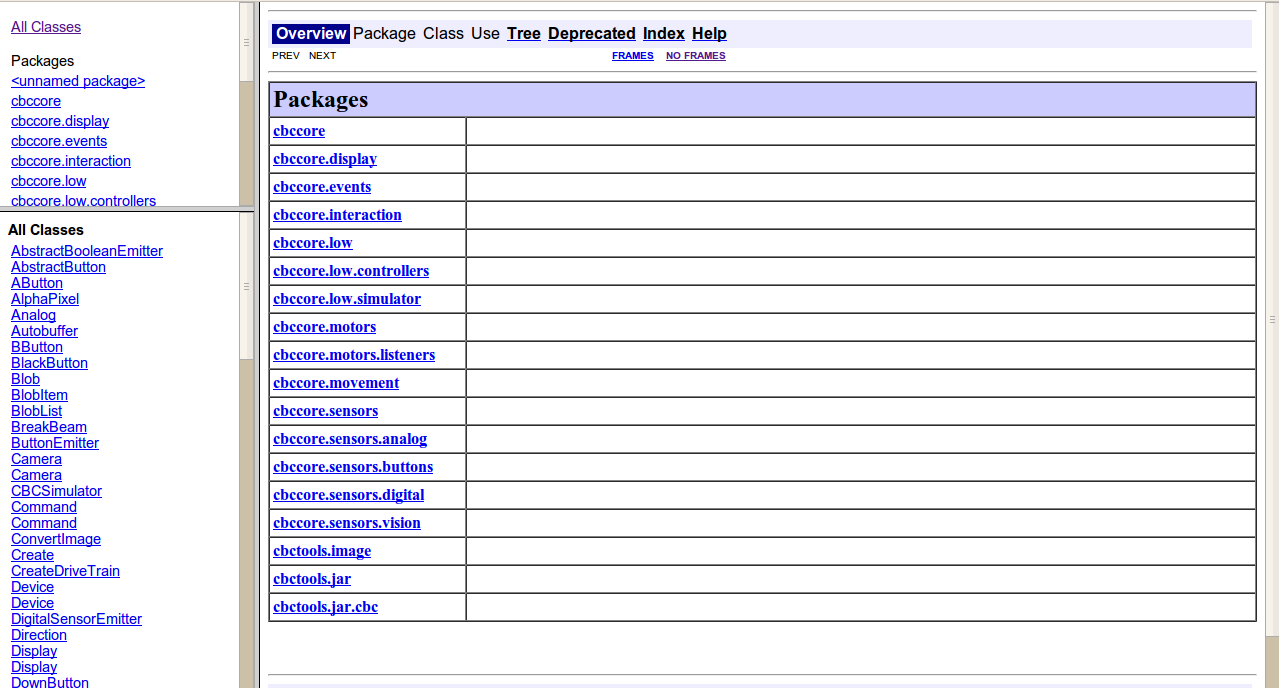
\includegraphics[width=\textwidth]{javadocs.png}
\caption{The CBCJVM JavaDocs. The top left frame contains CBCJVM specific packages. The bottom left frame contains CBCJVM specific classes. The large frame is used to display information about the currently selected package or class.}
\end{figure}

For regular users of Java, this should look familiar. That's because official JavaSE/ME/EE documentation is built using the same tool, JavaDoc. This generated documentation can be found on Oracle's website\urlfootnote{http://java.sun.com/javase/6/docs/api}. All of the classes and methods found there should be available on the CBC, with the notable exception of AWT/Swing (the packages are actually there, but the CBC lacks a windowing server, making them useless), and a few other minor features not yet available in JamVM/GNU-Classpath (such as \texttt{System.nanoTime()}).

\end{document}